\documentclass{article}
\usepackage{graphicx}
\usepackage{amsmath}
\usepackage{hyperref}
\graphicspath{ {images/} }
\title{Multi Agent System}
\date{March 2018}
\author{Ibis Prevedello}

\begin{document}
\maketitle

\section{Introduction}
The goal of this project is to implement a multi agent cooperation system to solve a given task, in this case manage a group of UAVs to automatically extinguish fires in a forest. The focus of this document is to present the algorithm developed, in particular the Contract Net Protocol (CNP) in order to assign the tasks for the UAVs. The source code for this project can be accessed from my \href{https://github.com/ibiscp/Fire-Extinguishers-Drones}{GitHub page}.

\section{Description of the problem}
The simulator is a representation of a forest where some fire outbreaks are being spread, as shown in image \ref{fig:fig1}. The fires and the drones start at random position and they need to communicate and decide which UAVs will help extinguish which fire as well where to move next and what to do if it cannot find any fire in the neighbor cells.

\begin{figure}[!ht]
\centering
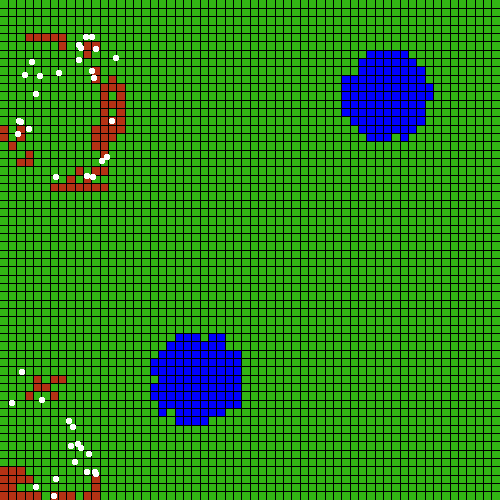
\includegraphics[scale=0.30]{environment}
\caption{Simulator screenshot}
\label{fig:fig1}
\end{figure}

It is important to mention that the UAVs can only see the status of the cell directly below them, so it is not possible to know if a move is worth or not (future cell is fire) without really going to the cell and checking it.

\section{Solution algorithm}
For the solution algorithm there are three basic steps implemented, the task assignment using Contract Net Protocol, the next cell selection (implementing a random walk) and the data sharing between the UAVs, all of which are described below.

\subsection{Task assignment}
For the task assigned it is implemented the Contract Net Protocol. In order to use it, first it is necessary to elect a manager, the closest UAV is automatically chosen as the manager if it is not already assined to any other task.

At the beggining, the managers send a proposal to all UAVs in the communication range with information about the fire outbreaks. The drones calculate an offer based on the cells with fire and the distance, with the following formula:

\[ offer = \dfrac{cells on fire}{distance} \]

When the manager receives all the proposals it assigns the task for the drones based on the offer received till all the drones necessary for the task are assigned.

It can happen that some drones are far from the managers and not in the range to receive or send a proposal, so in this case the drones chose a task randomly.

\subsection{Random walk}
The random walk is necessary for the UAVs to chose a next cell to visit. The UAVs are programed to chose a random cell in a 5x5 square from the current position, given that this new cell is inside the fores, smaller than the task radius and bigger than the task radius - 7. This value is chosen in order to not wast time doing random walk inside the an area that is already burned.

\subsection{Share data}
It was implemented a first version of sharing data, the drones are sharing their position with all the drones in the communication range if they see fire, so when a drone is lost, it can use this information of the closest drone in order to continue random walk from that position. It is important because when a group of drones is already finished to extinguish a fire in one place and there is no more fire nearby, they automatically move to the place where there is fire, and this behaviour can be easily seen with the simulation.

\section{Results}
To compile the results, a 50-iteration sequence was used to collect the data. The first result, shown in image \ref{fig:fig2}, is using 2 fire outbreaks with 40 UAVs with a communication range of 30 cells. It is possible to notice that with this number of fires and UAVs, there is a high number of normal cells, which means that the simulation finishes before burning it all, the drones are able to extinguish it.

\begin{figure}[!ht]
\centering
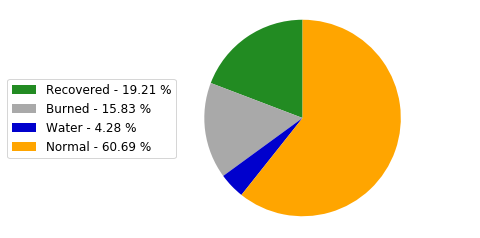
\includegraphics[scale=0.6]{fires_2_uavs_40_range_30}
\caption{Simulation with 2 fire outbreaks and 40 UAVs}
\label{fig:fig2}
\end{figure}

Changing the values for 3 fire outbreaks and only 20 UAVs with the same communication range, it is possible to see that the number of normal cells go to basically 0, which means the the drones were able to help extinguishing the fires but not avoiding it from spreading through the forest, as shown in image \ref{fig:fig3}.

\begin{figure}[!ht]
\centering
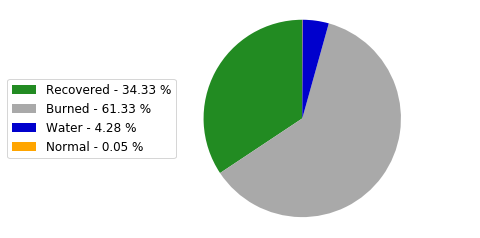
\includegraphics[scale=0.6]{fires_3_uavs_20_range_30}
\caption{Simulation with 3 fire outbreaks and 20 UAVs}
\label{fig:fig3}
\end{figure}

Now, using the same configuration as the first graph, however reducing the communication range to only 10 cells, it is possible to notice that the efficiency drops a lot. Image \ref{fig:fig4} shows that the UAVs are able to extinguish the fire before it spreads through the forest, but its result is notably worse when compared using a better communication range.

\begin{figure}[!ht]
\centering
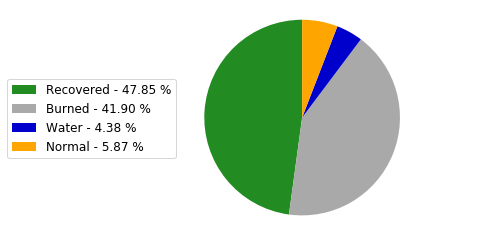
\includegraphics[scale=0.6]{fires_2_uavs_40_range_10}
\caption{Simulation with 2 fire outbreaks and 40 UAVs with low communication range}
\label{fig:fig4}
\end{figure}

\section{Conclusions}
It was really interesting to see and implement the Contract Net Protocol for multi agent cooperation system, and also study strategies to make it more efficient. The algorithm here presented is not perfect and a lot of things still could be done to have a better performance, however the results achieved are satisfatories and the goal of the project achieved.

For future work, it would be interesting to improve the data sharing, so the UAVs can share besides only their position, their internal map, so all other drones can update their knowledge and be more acertive when doing random walk.

\end{document}